\documentclass[10pt,twocolumn,letterpaper]{article}
\usepackage[utf8]{inputenc}
\usepackage[T1]{fontenc}
\usepackage{mathptmx}
\usepackage{courier}
\usepackage[top=0.75in,bottom=1in,left=0.65in,right=0.65in,columnsep=0.22in]{geometry}
\usepackage{amsmath,graphicx,booktabs,cite,float,stfloats}
%\usepackage[section]{placeins}
\usepackage[font=footnotesize,labelsep=period]{caption}
\usepackage[hidelinks]{hyperref}
\renewcommand{\figurename}{Fig.}
\renewcommand{\tablename}{TABLA}
\renewcommand{\thetable}{\Roman{table}}
\renewcommand{\refname}{Referencias}
\renewcommand{\abstractname}{Resumen}
\renewcommand{\thesection}{\Roman{section}}
\renewcommand{\thesubsection}{\Alph{subsection}}
\makeatletter
\renewcommand\section{\@startsection{section}{1}{\z@}{-1.5ex plus -.5ex minus -.2ex}{0.8ex}{\centering\normalfont\scshape}}
\renewcommand\subsection{\@startsection{subsection}{2}{\z@}{-1.2ex plus -.5ex minus -.2ex}{0.5ex}{\normalfont\itshape}}
\renewcommand{\@seccntformat}[1]{\csname the#1\endcsname.\quad}
\makeatother
\setlength{\parskip}{0pt}
\title{\Large Telemetría binaria BFSK en una planta de tratamiento de agua:\\ diseño y simulación de un enlace Tx--canal AWGN--Rx en GNU Radio\\ y prueba de un enlace SDR real con HackRF One}
\author{Jorge Mario Sánchez Arévalo (2234630), Sebastián Díaz Zuleta (2224034),\\ Ferney Esteban Vinasco Flórez (2202935)\\
\small Escuela de Ingenierías Eléctrica, Electrónica y de Telecomunicaciones, Universidad Industrial de Santander\\
\small Comunicaciones II (27145), Proyecto Integrador 2026, Grupo E1}
\date{}
\begin{document}
\maketitle

\begin{abstract}
\noindent Se diseña y simula un enlace de telemetría de baja velocidad para una planta de tratamiento de agua (escenario S5). Los nodos transmiten estados y medidas mediante BFSK de fase continua con $R_b=R_s=10$~kbit/s, $\Delta f=10$~kHz ($h=2$), $SPS=100$ y $f_s=1$~MS/s; el canal se modela como AWGN. Se propone un receptor no coherente formado por un filtro de selección de canal, un discriminador de frecuencia, un integrador por símbolo, un muestreo de una muestra por símbolo y un decisor con umbral cero. Se comparan dos receptores en cuatro niveles de ruido. Sin filtro de canal, el discriminador entra en la región de umbral y la BER alcanza $2.4\times10^{-2}$ en la prueba media y $1.3\times10^{-1}$ en la fuerte. Con el filtro, la BER es nula en las cuatro pruebas y la curva de error se desplaza unos 13~dB hacia relaciones $E_b/N_0$ menores. Además, en el laboratorio se montó un enlace real entre dos computadores con HackRF One y flujogramas 16-QAM ($f_c=960$~MHz, $R_b=32$~kbit/s, tramas con CRC-32). El receptor recuperó con CRC válido el mensaje ``El Pensador'' y reconstruyó por franjas el 15~\% del logo de la UIS, con un EVM de 16.7~\% (MER $\approx$ 15.5~dB).
\end{abstract}

\noindent\textbf{\small Palabras clave:} \small BFSK, CPFSK, discriminador de frecuencia, efecto umbral, GNU Radio, HackRF One, 16-QAM, SDR, telemetría.\normalsize

\section{Introducción y escenario}
Las plantas de tratamiento de agua supervisan niveles de tanques, estados de bombas y posiciones de válvulas desde una sala de control. Cablear cada punto es costoso, por lo que es común usar nodos inalámbricos de bajo consumo en bandas ISM sub-GHz, donde predominan las modulaciones 2-FSK y GFSK \cite{st_subghz}. Un ejemplo normalizado es Wireless M-Bus (EN~13757-4), que emplea FSK con índices de modulación de 0.8 a 1.6 para lectura remota de medidores \cite{an0987}.

El escenario elegido (Fig.~\ref{fig:escenario}) contiene tres nodos (Tx1--Tx3) a distancias de 80 a 300~m del receptor. El fenómeno que degrada el enlace es la combinación de atenuación por distancia y ruido térmico del receptor: cuando la potencia recibida se acerca al piso de ruido, la señal compleja recibida se modela como $r[n]=x[n]+w[n]$, con $w[n]$ ruido gaussiano blanco complejo (AWGN). La información a transmitir son tramas cortas de estados binarios y medidas lentas.

\begin{figure}[H]
\centering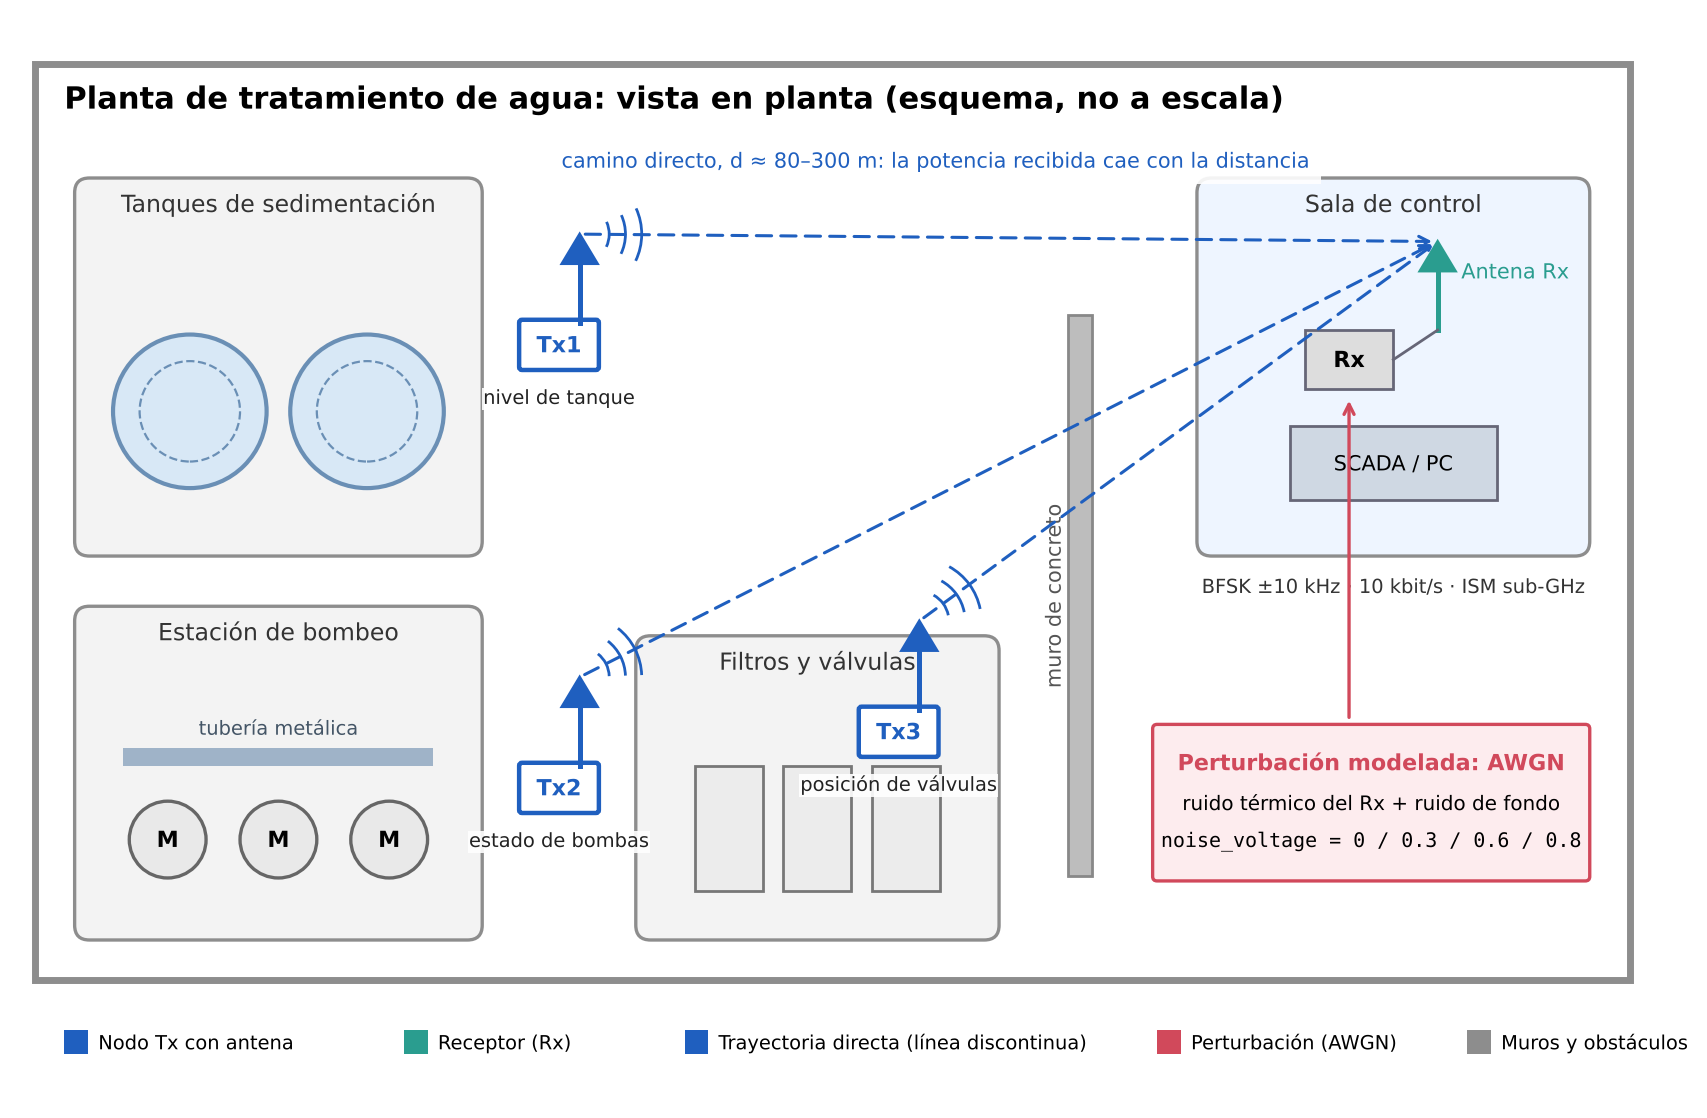
\includegraphics[width=\columnwidth]{figures/escenario/fig01_escenario_contextual.png}
\caption{Escenario contextual: nodos Tx con antena, trayectorias directas hacia el receptor de la sala de control, obstáculos y fuente de degradación modelada (AWGN).}
\label{fig:escenario}
\end{figure}

\section{Fundamento teórico}
\subsection{BFSK de fase continua}
Cada bit $b_k$ se mapea a $m_k=2b_k-1\in\{-1,+1\}$ y se mantiene durante $T_s$. La envolvente compleja generada por el modulador de frecuencia es
\begin{equation}
x[n]=e^{j\phi[n]},\qquad \phi[n]=\phi[n-1]+\frac{2\pi\Delta f}{f_s}\,m[n],
\end{equation}
de modo que la frecuencia instantánea vale $\pm\Delta f$ y la fase es continua. El índice de modulación es $h=2\Delta f/R_s$; para $h$ entero los tonos son ortogonales sobre un periodo de símbolo \cite{proakis}. El ancho de banda se aproxima con la regla de Carson, $B\approx2(\Delta f+R_s)$ \cite{sklar}.

\subsection{Detección por discriminador y efecto umbral}
El discriminador estima la frecuencia instantánea a partir del giro de fase entre muestras consecutivas:
\begin{equation}
y[n]=\frac{f_s}{2\pi\Delta f}\arg\!\left(r[n]\,r^{*}[n-1]\right)\approx m[n]+\text{ruido}.
\end{equation}
Es un detector no coherente: no necesita recuperar la fase de la portadora. Su desventaja es el efecto umbral: cuando la relación portadora/ruido a su entrada cae por debajo de unos 10~dB, el ruido supera momentáneamente a la señal, la fase salta casi $2\pi$ y aparecen impulsos (\emph{clicks}) en la salida \cite{ahaneku}. Por eso importa el ancho de banda de ruido que ve el discriminador, no solo $E_b/N_0$.

\section{Diseño del sistema y parámetros}
Se seleccionó BFSK por su envolvente constante (amplificadores no lineales eficientes), su detección no coherente y su robustez frente a variaciones de amplitud. Se consideró BPSK, que requiere unos 4~dB menos de $E_b/N_0$ para BER $=10^{-5}$ y ocupa $(1+\beta)R_s\approx13.5$~kHz con RRC ($\beta=0.35$), pero exige recuperar portadora y fase con osciladores de bajo costo y presenta ambigüedad de $180^\circ$; a 10~kbit/s esa complejidad no se justifica. La Tabla~\ref{tab:param} resume los parámetros.

\begin{table}[!htb]
\centering\footnotesize
\caption{Parámetros del sistema}
\label{tab:param}
\begin{tabular}{@{}lll@{}}
\toprule
Parámetro & Valor & Relación / justificación\\
\midrule
$M$, $k$ & 2, 1 bit/símb. & $k=\log_2M$\\
$R_s$ & 10 kbaud & $f_s/SPS$\\
$R_b$ & 10 kbit/s & $R_s\cdot k$; 40 nodos usan 51\,\%\\
$SPS$ & 100 & resolución del ojo y de $f_{inst}$\\
$f_s$ & 1 MS/s & $R_s\cdot SPS$; $f_s/B=25$\\
$\Delta f$ & 10 kHz & base: 20 kHz\\
$h$ & 2 & $2\Delta f/R_s$, tonos ortogonales\\
$B$ & $\approx$40 kHz & Carson; 60 kHz con la base\\
noise\_voltage & 0 / 0.3 / 0.6 / 0.8 & pruebas A--D\\
\bottomrule
\end{tabular}
\end{table}

La desviación se redujo de 20 a 10~kHz: con $h=1$ el espectro sería más compacto, pero la excursión del discriminador sería menor y más sensible al ruido; con $h=4$ el ancho de banda llega a 60~kHz (Fig.~\ref{fig:psddf}). Se conservan $f_s$ y $SPS$ de la base para mantener la comparabilidad con las guías anteriores.

\begin{figure}[H]
\centering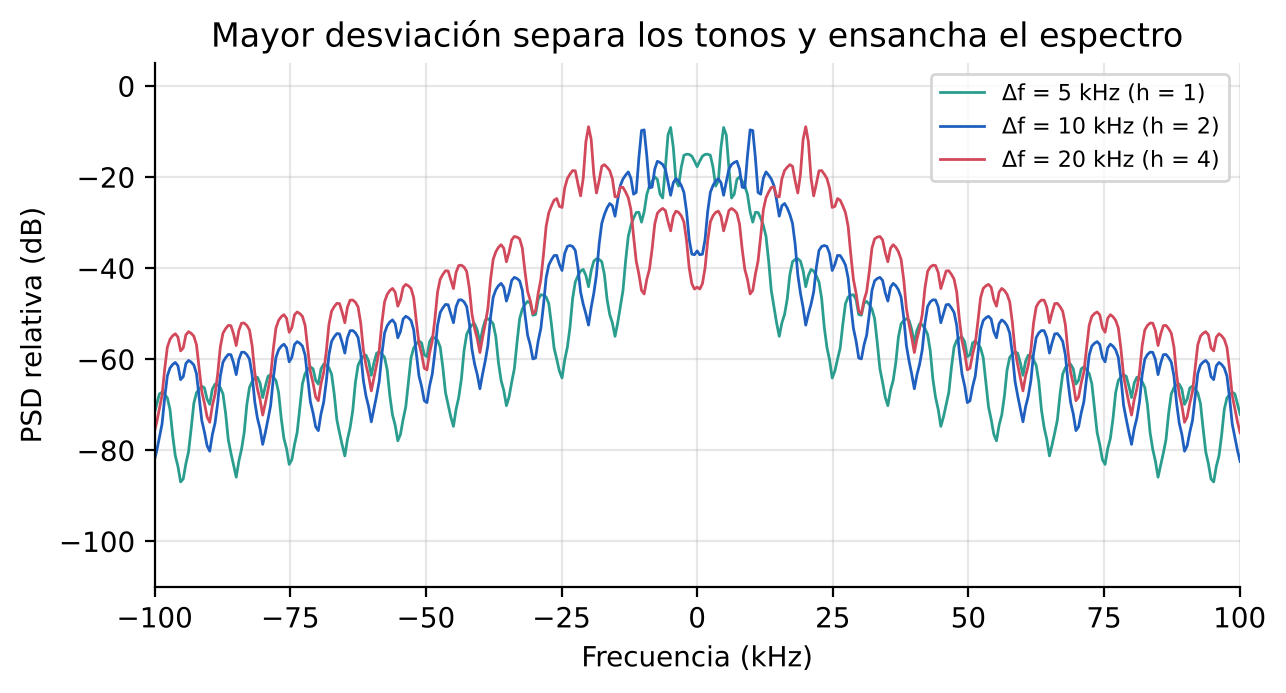
\includegraphics[width=0.9\columnwidth]{figures/psd/fig12_psd_vs_desviacion.png}
\caption{PSD de la señal transmitida para $\Delta f=5$, 10 y 20~kHz con $R_s=10$~kbaud.}
\label{fig:psddf}
\end{figure}

La potencia de la señal es unitaria y el bloque Channel Model añade ruido complejo de potencia $\sigma^2$, con $\sigma=$~noise\_voltage, en todo el ancho $f_s$. Entonces
\begin{equation}
\mathrm{SNR}_{f_s}=\frac{1}{\sigma^2},\qquad \frac{E_b}{N_0}=\frac{f_s}{R_b\,\sigma^2}=\frac{100}{\sigma^2}.
\end{equation}
Si el discriminador recibe la señal sin filtrar, opera con la SNR medida en 1~MHz; con un filtro de 40~kHz la SNR a su entrada mejora $10\log_{10}(10^6/4\times10^4)\approx14$~dB.

\section{Metodología de simulación en GNU Radio}
Se partió del archivo base \path{Guia2_BASE_FSK_Canal_Discriminador.grc} y se creó \path{S5_BFSK_TxCanalRx_GrupoE1.grc} (Fig.~\ref{fig:diag}). El transmisor no cambia: Vector Source (16 bits), Chunks to Symbols ($0\to-1$, $1\to+1$), Repeat ($\times SPS$), Frequency Mod ($k=2\pi\Delta f/f_s$) y Throttle. El receptor añadido tiene cinco etapas:
\begin{enumerate}
\item \emph{Filtro de selección de canal}: FIR paso bajo, Hamming, corte 20~kHz, transición 10~kHz (241 coeficientes, retardo de 120 muestras). Una mezcla ponderada (Multiply Const con pesos $1-r$ y $r$, más un Add) elige R1 (sin filtro, con un Delay de 120 muestras para igualar latencias) o R2 (con filtro); ambos caminos procesan siempre la señal, de modo que cambiar de receptor no desalinea los flujos.
\item \emph{Discriminador}: Quadrature Demod con ganancia $f_s/(2\pi\Delta f)$.
\item \emph{Filtro acoplado al pulso}: Moving Average de longitud $SPS$ y escala $1/SPS$ (integrar y descargar).
\item \emph{Muestreo}: Skip Head de $120 \bmod 100=20$ muestras y Keep One in N con $N=100$, que conserva la última muestra de cada ventana, donde el ojo está más abierto.
\item \emph{Decisión}: Binary Slicer con umbral 0, umbral de máxima verosimilitud para niveles simétricos equiprobables.
\end{enumerate}
La validación compara, con XOR, los bits recuperados con la referencia transmitida retardada $D_b=\lfloor120/100\rfloor=1$~bit, y estima la BER con un promedio móvil de 1000 bits. Se varió únicamente noise\_voltage en cuatro niveles: A (0), B (0.3), C (0.6) y D (0.8). Las métricas cuantitativas se obtuvieron con un modelo numérico en Python que reproduce la misma cadena, los mismos retardos y la misma regla de muestreo del flujograma, con $10^5$ bits por prueba, y se verificaron ejecutando el flujograma en GNU Radio 3.10.12.

\begin{figure*}[!t]
\centering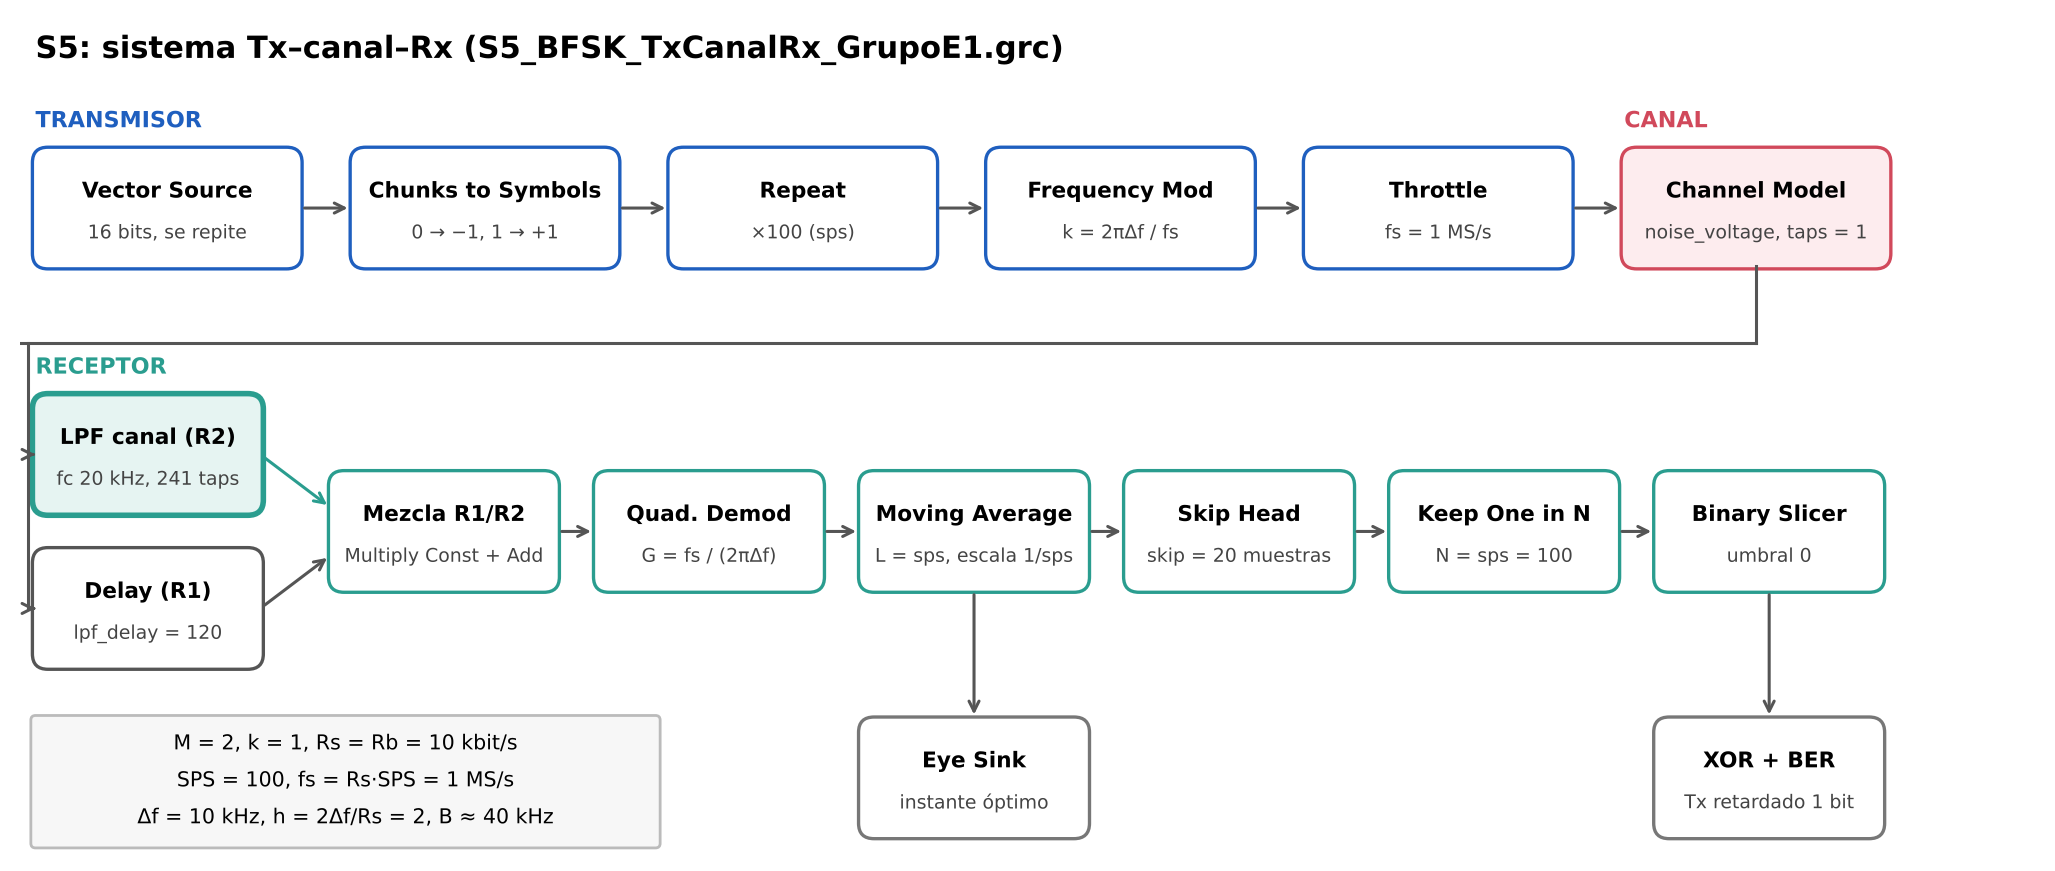
\includegraphics[width=0.92\textwidth]{figures/diagramas_tecnicos/fig02_diagrama_tecnico_tx_canal_rx.png}
\caption{Diagrama técnico del sistema implementado en el GRC: transmisor CPFSK, canal AWGN, receptores R1 y R2, observación (Eye Sink) y validación por BER.}
\label{fig:diag}
\end{figure*}

\section{Resultados}
\subsection{Referencia (prueba A)}
La PSD de la Fig.~\ref{fig:psdA} muestra dos máximos en $\pm10$~kHz y lóbulos que decaen fuera de la banda de Carson. El discriminador reproduce la onda $\pm1$ sin errores y el ojo está totalmente abierto en ambos receptores (Fig.~\ref{fig:ojos}).

\begin{figure}[H]
\centering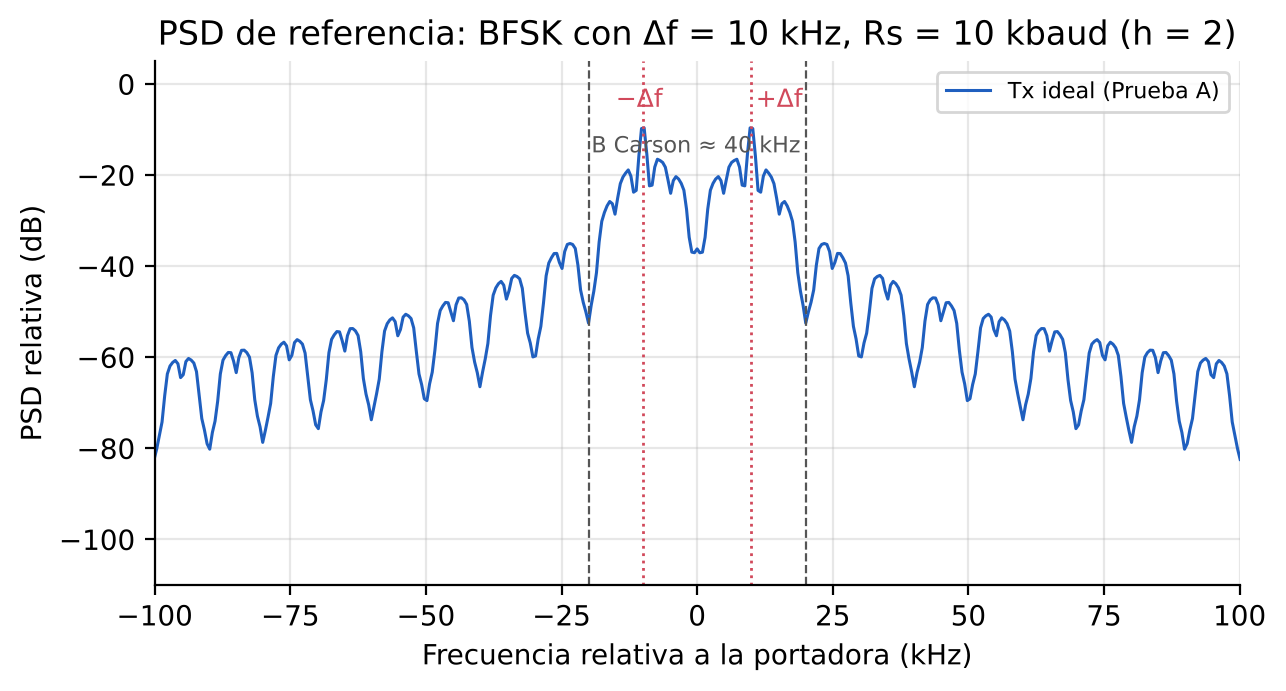
\includegraphics[width=0.9\columnwidth]{figures/psd/fig05_psd_referencia_A.png}
\caption{PSD de referencia (prueba A). Líneas punteadas: tonos en $\pm\Delta f$; discontinuas: límites de Carson.}
\label{fig:psdA}
\end{figure}

\subsection{Pruebas con ruido}
La Tabla~\ref{tab:pruebas} resume la BER del modelo. En GNU Radio, el Number Sink (ventana de 1000 bits) mostró A y B sin errores; en C, R1 entre 0.022 y 0.033 y R2 nula; en D, R1 entre 0.155 y 0.169 y R2 nula. La Fig.~\ref{fig:gr} reúne las capturas de GNU Radio de la prueba C: con R1 la salida del discriminador está dominada por clicks y el ojo se cierra; con R2 la frecuencia instantánea sigue la referencia y el ojo permanece abierto.

\begin{figure*}[!t]
\centering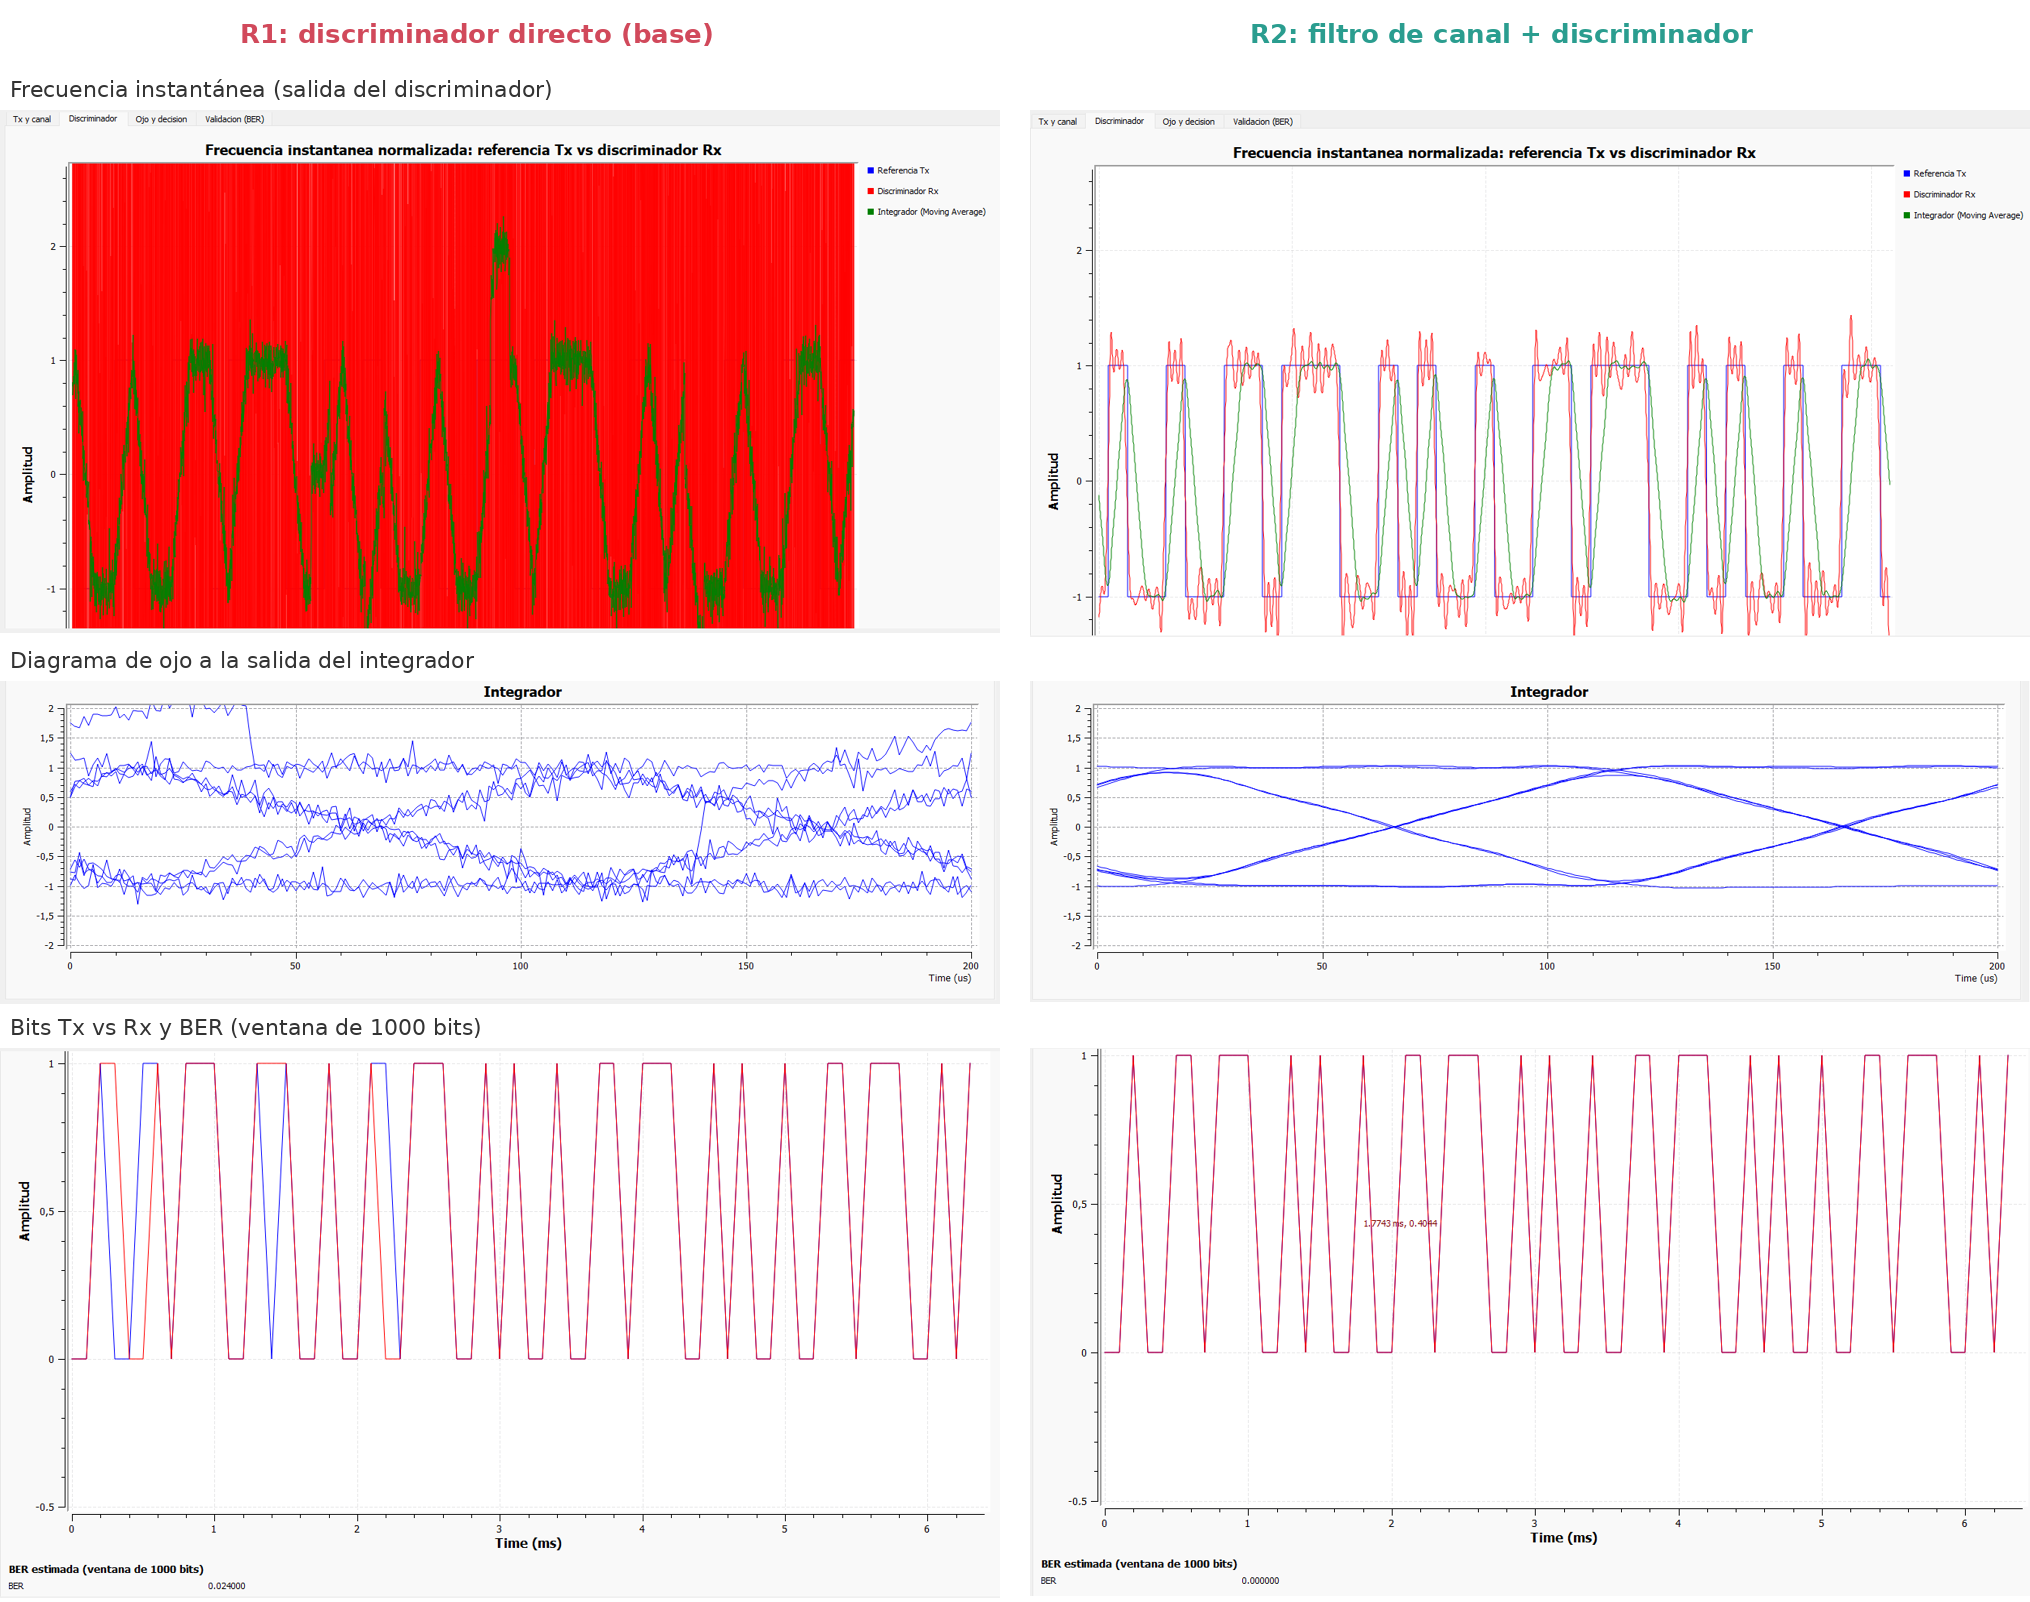
\includegraphics[width=0.72\textwidth]{figures/gnuradio/fig14_gnuradio_C_R1_vs_R2.png}
\caption{Capturas de GNU Radio 3.10.12 en la prueba C (noise\_voltage $=0.6$). Izquierda: R1; derecha: R2. Filas: frecuencia instantánea, diagrama de ojo y bits Tx/Rx con la BER estimada (0.024 y 0).}
\label{fig:gr}
\end{figure*}
 La Fig.~\ref{fig:psdCD} muestra que el AWGN eleva un piso plano en toda la banda de 1~MHz, mientras que el filtro de canal elimina el ruido fuera de $\pm20$~kHz. La Fig.~\ref{fig:finst} compara la frecuencia instantánea en la prueba C: en R1 la salida del discriminador está dominada por clicks; en R2 conserva la forma de los símbolos.

\begin{table}[!htb]
\centering\footnotesize
\caption{Plan de pruebas y BER obtenida ($10^5$ bits, $\Delta f=10$~kHz)}
\label{tab:pruebas}
\begin{tabular}{@{}cccccc@{}}
\toprule
Prueba & $\sigma$ & SNR$_{1\,\mathrm{MHz}}$ & $E_b/N_0$ & BER R1 & BER R2\\
\midrule
A & 0 & $\infty$ & $\infty$ & 0 & 0\\
B & 0.3 & 10.5 dB & 30.5 dB & 0 & 0\\
C & 0.6 & 4.4 dB & 24.4 dB & $2.4\times10^{-2}$ & 0\\
D & 0.8 & 1.9 dB & 21.9 dB & $1.3\times10^{-1}$ & 0\\
\bottomrule
\end{tabular}
\end{table}

\begin{figure*}[!t]
\centering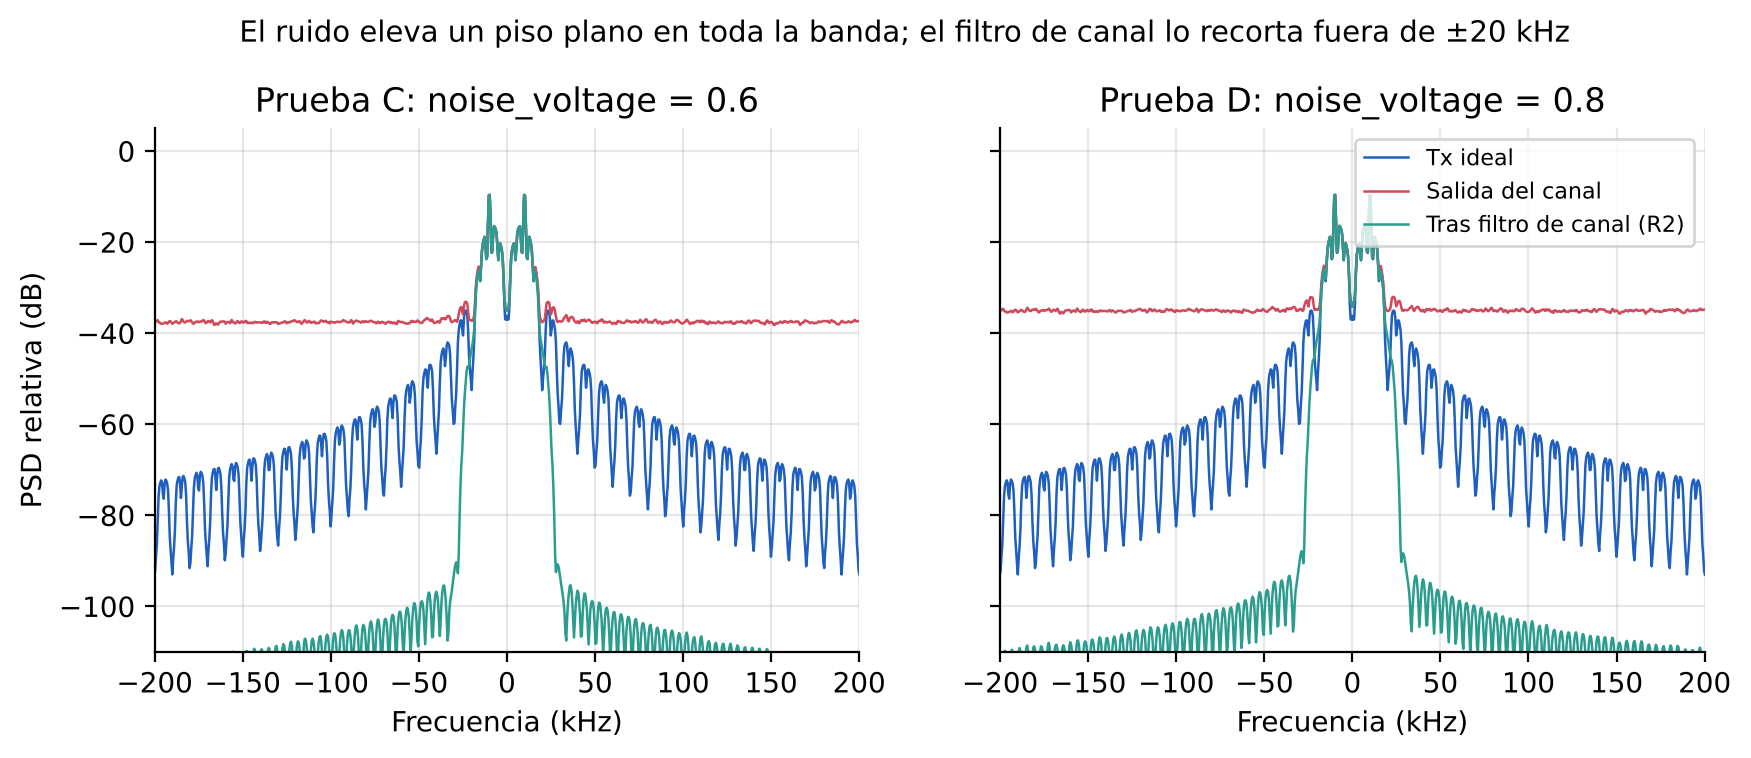
\includegraphics[width=0.75\textwidth]{figures/psd/fig06_psd_perturbacion_C_D.png}
\caption{PSD en las pruebas C y D: señal transmitida, salida del canal y entrada al discriminador en R2.}
\label{fig:psdCD}
\end{figure*}

\begin{figure}[H]
\centering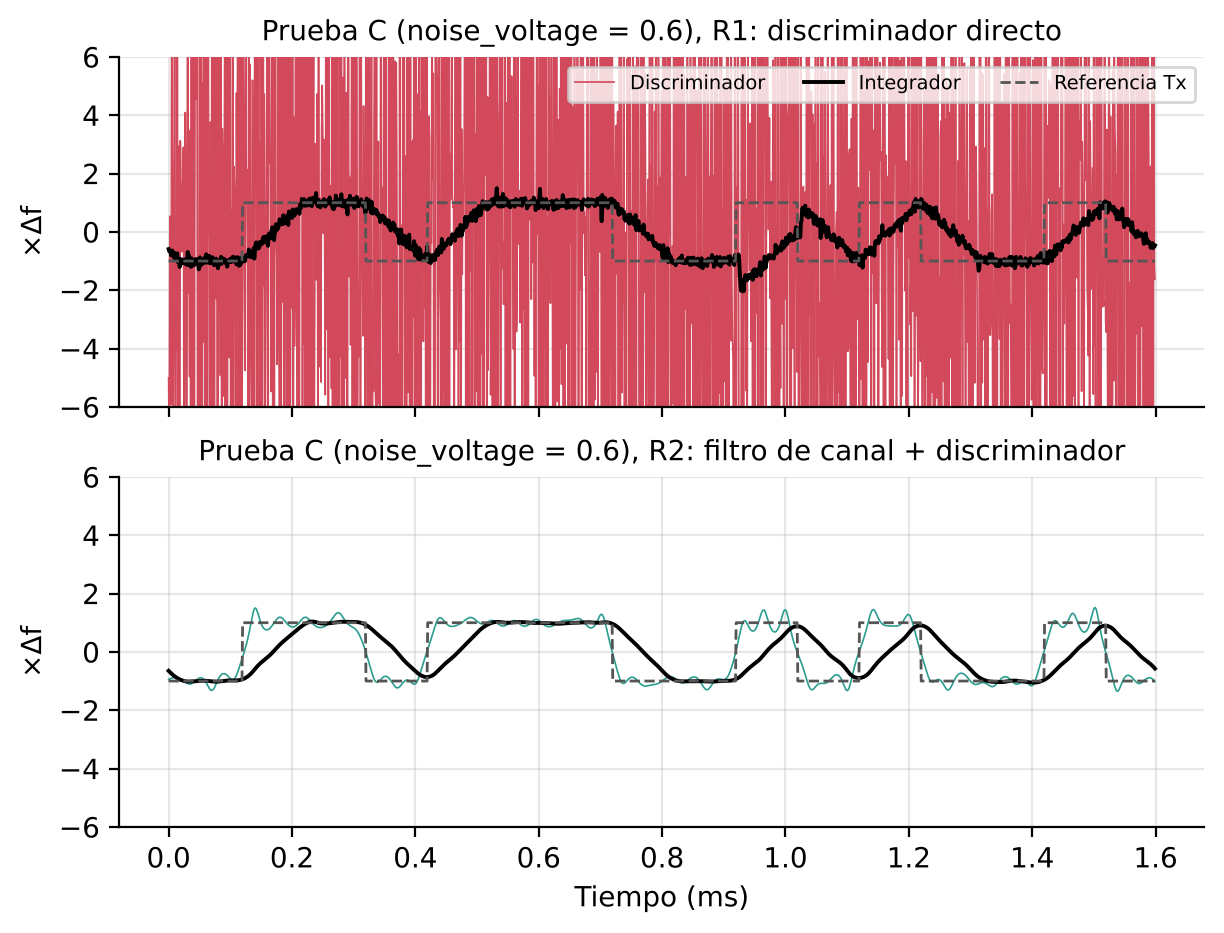
\includegraphics[width=0.9\columnwidth]{figures/constelacion_o_fsk/fig08_frecuencia_instantanea_C_R1_R2.png}
\caption{Frecuencia instantánea normalizada en la prueba C: salida del discriminador, salida del integrador y referencia Tx.}
\label{fig:finst}
\end{figure}




\section{Análisis de resultados}
\begin{figure}[H]
\centering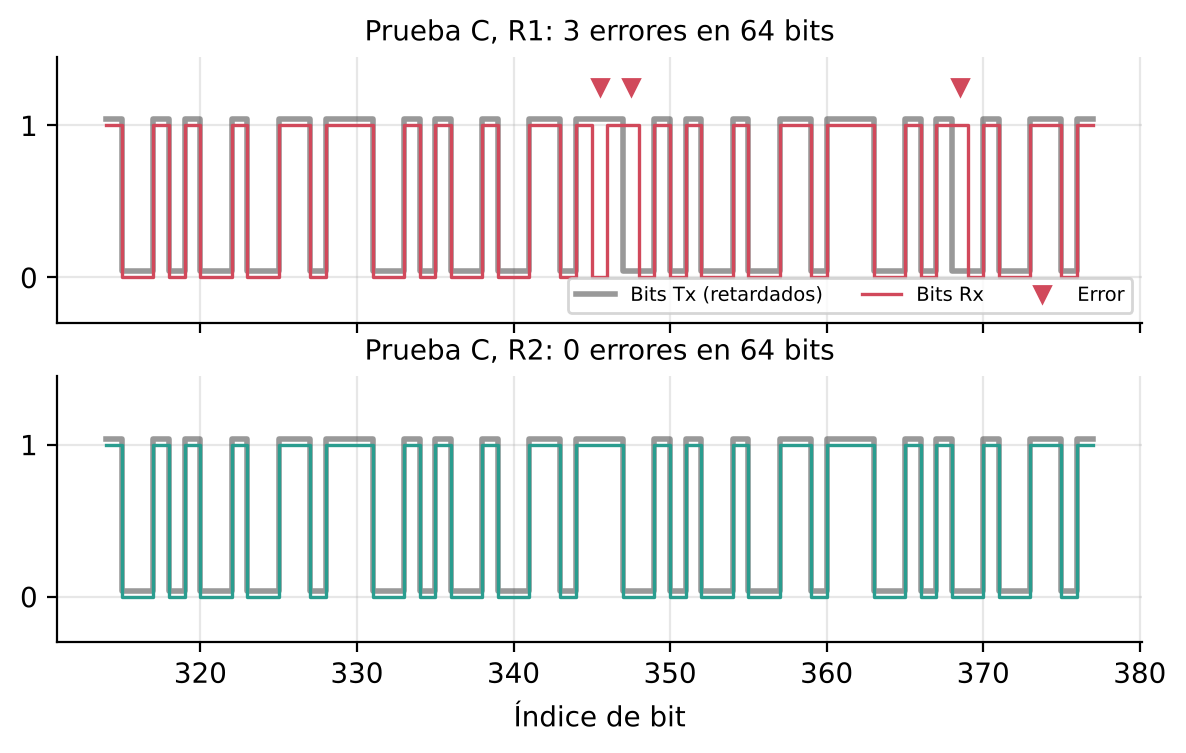
\includegraphics[width=0.9\columnwidth]{figures/constelacion_o_fsk/fig10_bits_tx_rx_C.png}
\caption{Bits transmitidos (retardados un bit) y recuperados en la prueba C. Los triángulos marcan los errores de R1.}
\label{fig:bits}
\end{figure}

\begin{figure*}[!t]
\centering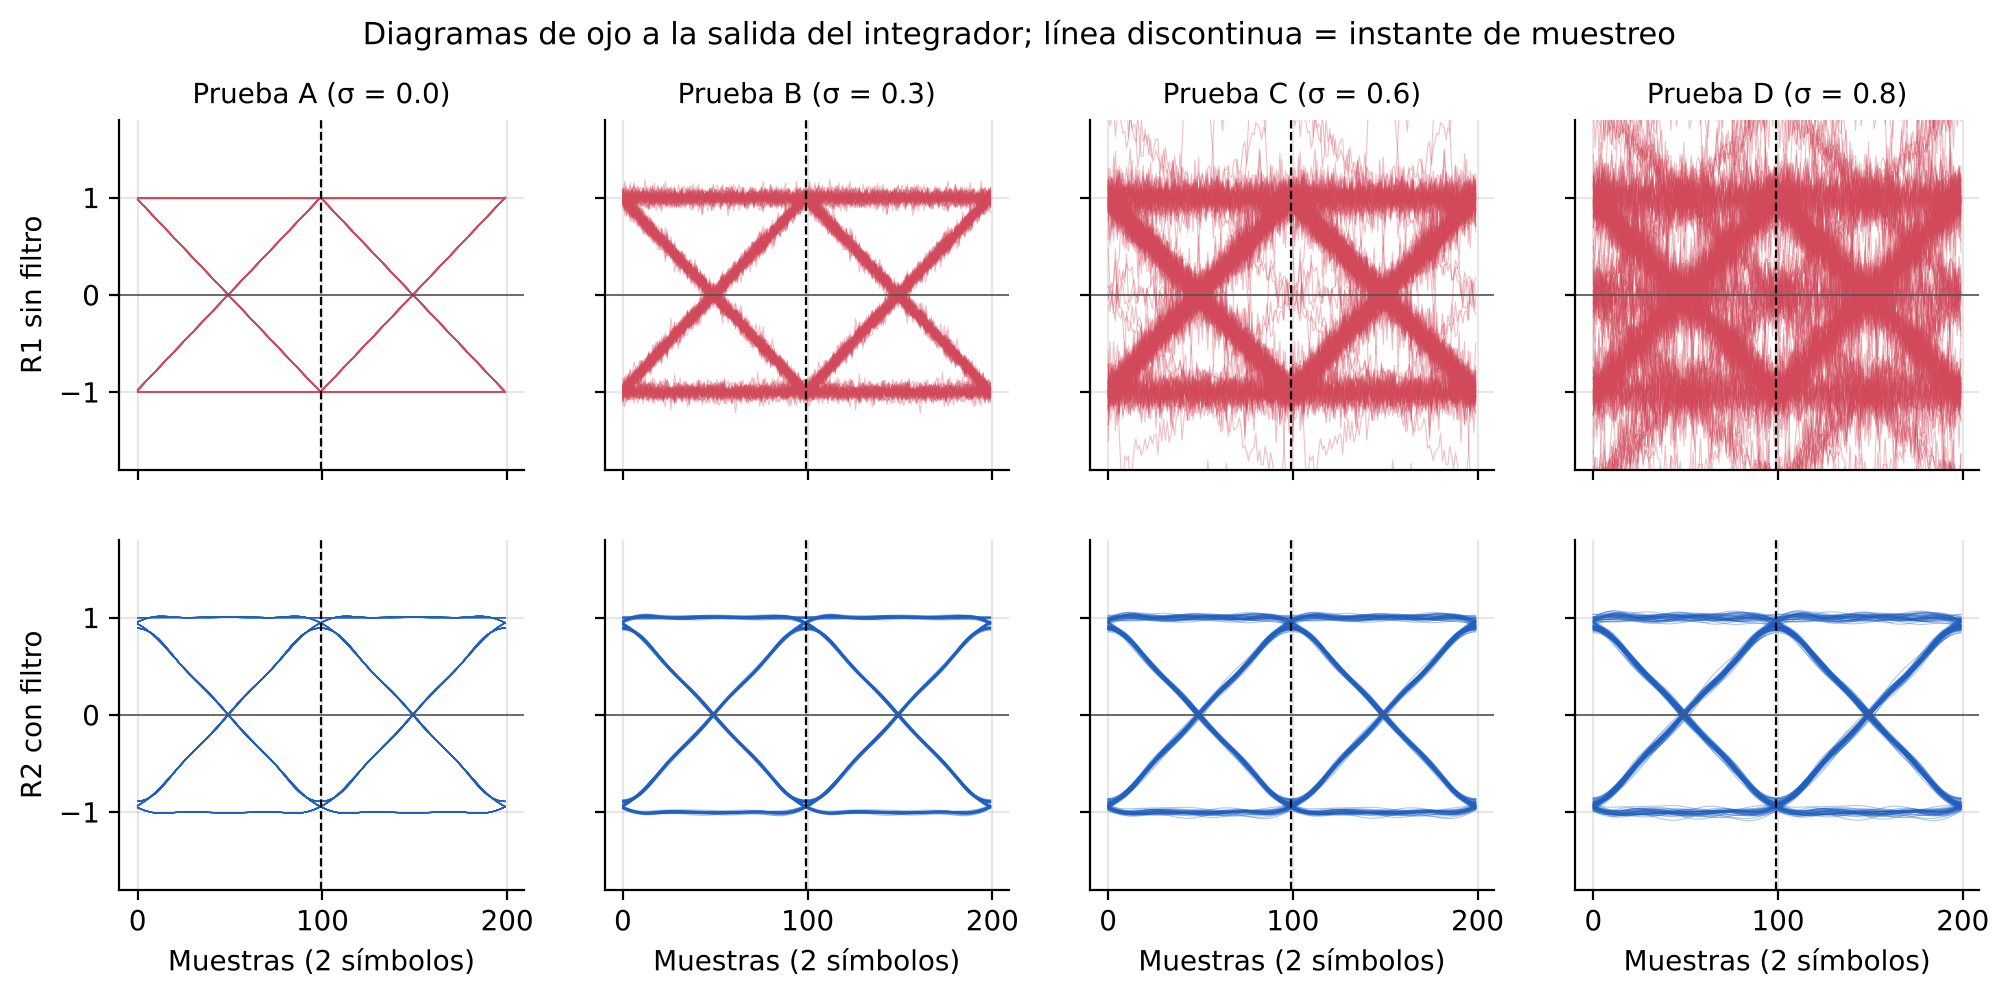
\includegraphics[width=0.78\textwidth]{figures/constelacion_o_fsk/fig09_diagramas_de_ojo.png}
\caption{Diagramas de ojo a la salida del integrador para las pruebas A--D. Fila superior: R1; inferior: R2. La línea discontinua marca el instante de muestreo.}
\label{fig:ojos}
\end{figure*}

\textbf{Efecto umbral.} En la prueba C la $E_b/N_0$ es de 24.4~dB; un detector óptimo no cometería errores. Sin embargo, R1 registra una BER de $2.4\times10^{-2}$ porque su discriminador opera con 4.4~dB de SNR en 1~MHz, por debajo del umbral de unos 10~dB \cite{ahaneku}. El integrador promedia el ruido gaussiano pero no elimina los clicks, que se trasladan a errores (Fig.~\ref{fig:bits}). En R2 la SNR a la entrada del discriminador es de unos 18~dB y no hay errores.

\textbf{Diagrama de ojo e ISI.} La ISI de R1 y R2 en la prueba A proviene de la memoria del integrador y, en R2, de la respuesta del filtro de canal; ambas se anulan en el instante de muestreo elegido, donde la ventana cubre exactamente un símbolo. En R2 el máximo es ligeramente menor que 1 (Fig.~\ref{fig:ojos}) porque el filtro suaviza las transiciones de frecuencia, pero el margen frente al umbral sigue siendo amplio.

\begin{figure}[H]
\centering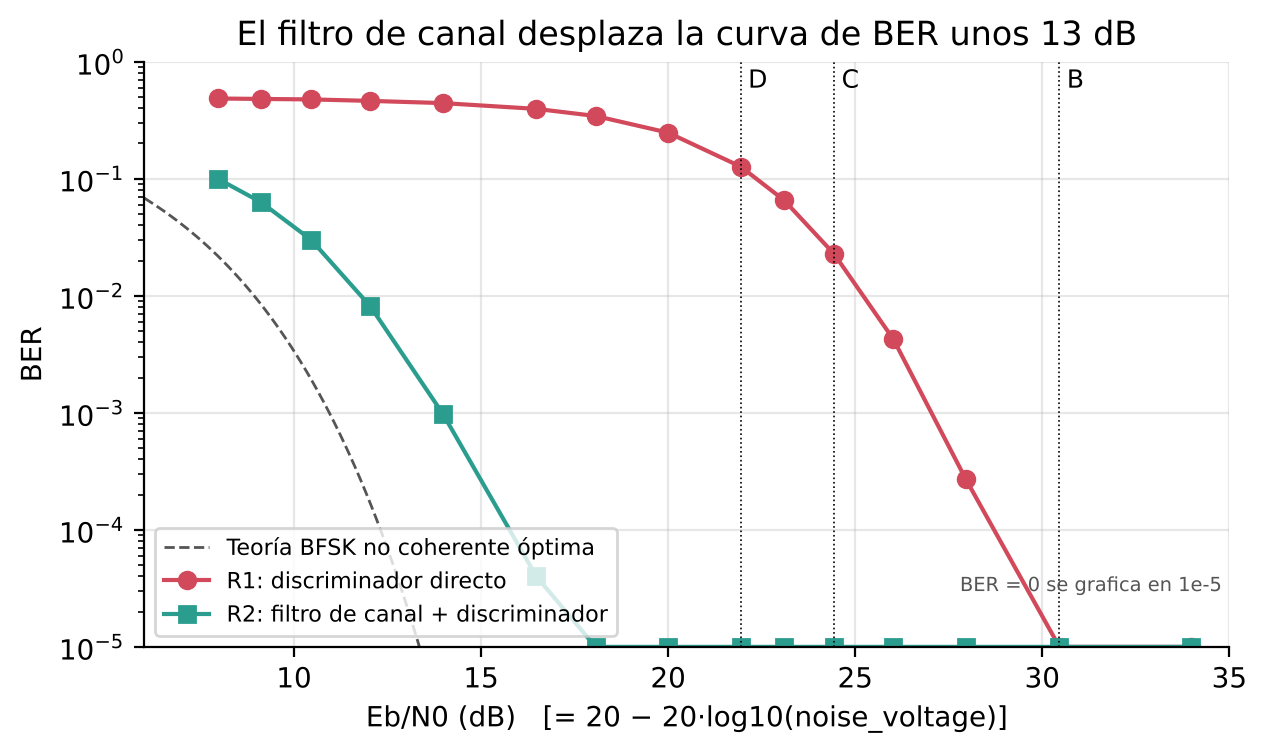
\includegraphics[width=0.9\columnwidth]{figures/constelacion_o_fsk/fig11_ber_vs_ruido.png}
\caption{BER frente a $E_b/N_0$ para R1 y R2, con la curva teórica de BFSK no coherente óptima. Las líneas punteadas indican las pruebas B--D.}
\label{fig:ber}
\end{figure}

\textbf{Margen del receptor propuesto.} La Fig.~\ref{fig:ber} muestra que el filtro desplaza la curva unos 13~dB. R2 se degrada solo con noise\_voltage $\ge1.5$ (BER $=4\times10^{-5}$) y alcanza $3\times10^{-2}$ con $\sigma=3$ ($E_b/N_0=10.5$~dB). Persiste una brecha de unos 3--4~dB respecto al detector no coherente óptimo, atribuible al umbral residual del discriminador y a que el filtro de 40~kHz es más ancho que el ancho de banda de ruido del filtro acoplado ideal.

\textbf{Desviación de frecuencia.} Con R1 y $\sigma=0.6$, la BER pasa de $4.1\times10^{-2}$ ($h=1$) a $2.2\times10^{-2}$ ($h=2$) y $6\times10^{-4}$ ($h=4$): mayor desviación da más margen al discriminador a costa de ancho de banda. Con el filtro de canal, $h=2$ ya es suficiente, por lo que no se necesita el ancho de banda de $h=4$.

\textbf{Relación con la aplicación.} El nodo más lejano de la planta equivale a la prueba D: con un receptor que solo usara el discriminador de la base, se perdería más del 10\,\% de los bits. El receptor propuesto mantiene el enlace sin errores con el mismo transmisor, lo que permite ubicar nodos más lejos o reducir la potencia de transmisión y prolongar la vida de las baterías.

\section{Prueba en hardware SDR con HackRF One}
El 5 de noviembre de 2026 se llevó un enlace digital a radios reales. Se usaron dos HackRF One, cada uno conectado a un computador distinto: otro grupo ejecutó el transmisor y nuestro grupo, el receptor. Los flujogramas del laboratorio emplean 16-QAM; la prueba pone en un canal físico los mismos elementos estudiados en la simulación: filtrado, sincronización, ruido y verificación de bits. Se hicieron dos pruebas: un mensaje de texto y una imagen.

\subsection{Montaje y parámetros}
Los dos HackRF, con antena, se ubicaron a poca distancia sobre las mesas del laboratorio y se conectaron por USB a sus computadores (Fig.~\ref{fig:montaje}). El enlace fue por aire. La Tabla~\ref{tab:paramhw} resume los parámetros de los flujogramas.

\begin{figure}[H]
\centering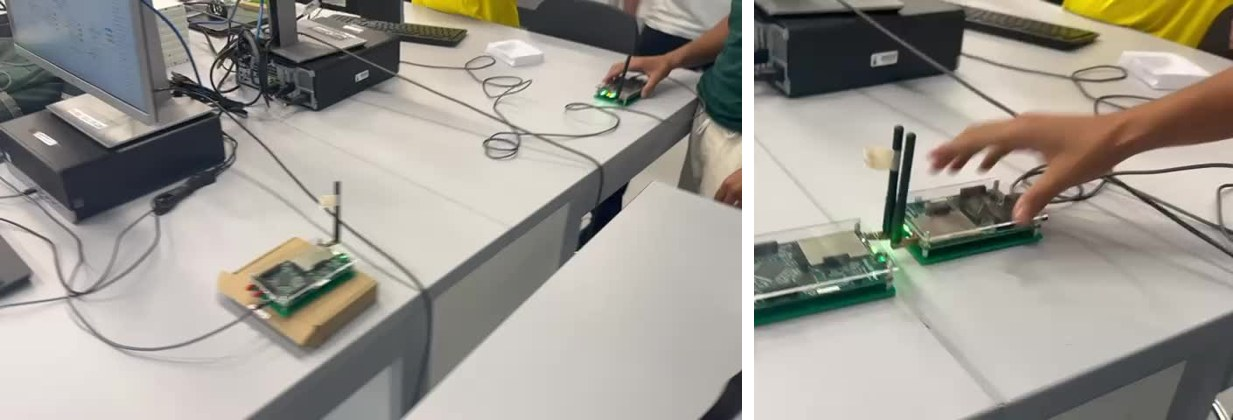
\includegraphics[width=\columnwidth]{figures/hardware_sdr/f4_montaje.jpg}
\caption{Montaje: HackRF One transmisor y receptor, cada uno conectado a su computador.}
\label{fig:montaje}
\end{figure}

\begin{table}[!htb]
\centering\footnotesize
\caption{Parámetros del enlace con HackRF One}
\label{tab:paramhw}
\begin{tabular}{@{}lll@{}}
\toprule
Parámetro & Valor & Relación\\
\midrule
Modulación & 16-QAM, Gray & $k=\log_2 16=4$\\
$R_s$ & 8 kbaud & \\
$R_b$ & 32 kbit/s & $R_s\cdot k$\\
SPS & 8 & \\
Tasa de banda base & 64 kS/s & $R_s\cdot SPS$\\
Tasa del radio & 2 MS/s & $64\text{k}\cdot125/4$\\
Filtro & RRC, $\beta=0.5$, 11 símb. & \\
Ancho de banda & $\approx$12 kHz & $(1+\beta)R_s$\\
$f_c$ & 960 MHz & \\
Desfase del LO & 200 kHz & evita el pico DC\\
Tx: amplitud / IF & 0.15 / 20 dB & \\
Rx: LNA / VGA & 16 / 20 dB & \\
\bottomrule
\end{tabular}
\end{table}

El HackRF tiene una componente espuria en el centro de su banda por fuga del oscilador local \cite{hackrf}. Para evitarla, el transmisor sintoniza $f_c-200$~kHz y desplaza digitalmente la señal $+200$~kHz, de modo que sale en 960~MHz; el receptor sintoniza $f_c+200$~kHz y la devuelve a banda base. Por eso la I/Q que llega al HackRF transmisor oscila a 200~kHz (Fig.~\ref{fig:txgui}).

\subsection{Transmisor y receptor}
\emph{Transmisor:} fuente de tramas (bloque Python) $\rightarrow$ Chunks to Symbols (16-QAM con $E_s=1$) $\rightarrow$ filtro RRC interpolador ($\times8$) $\rightarrow$ escala 0.15 $\rightarrow$ Rational Resampler 125/4 $\rightarrow$ Frequency Xlating ($+200$~kHz) $\rightarrow$ Osmocom Sink (Fig.~\ref{fig:txflujo}). Cada trama tiene un preámbulo pseudoaleatorio de 64 símbolos, conocido por Tx y Rx, los datos con su CRC-32 y una guarda de 24 símbolos.

\emph{Receptor:} Osmocom Source $\rightarrow$ Frequency Xlating $\rightarrow$ Rational Resampler 4/125 $\rightarrow$ AGC $\rightarrow$ FLL Band-Edge (corrige el desfase de frecuencia entre radios) $\rightarrow$ Polyphase Clock Sync con RRC de 32 filtros (filtro acoplado y sincronismo de símbolo) $\rightarrow$ AGC de símbolos $\rightarrow$ Constellation Receiver (lazo de portadora y decisión) $\rightarrow$ medidor de tramas. El medidor busca el preámbulo en las cuatro rotaciones posibles (0, 90, 180 y 270°), corrige la ambigüedad de fase, verifica el CRC y calcula BER y EVM.

\begin{figure*}[!t]
\centering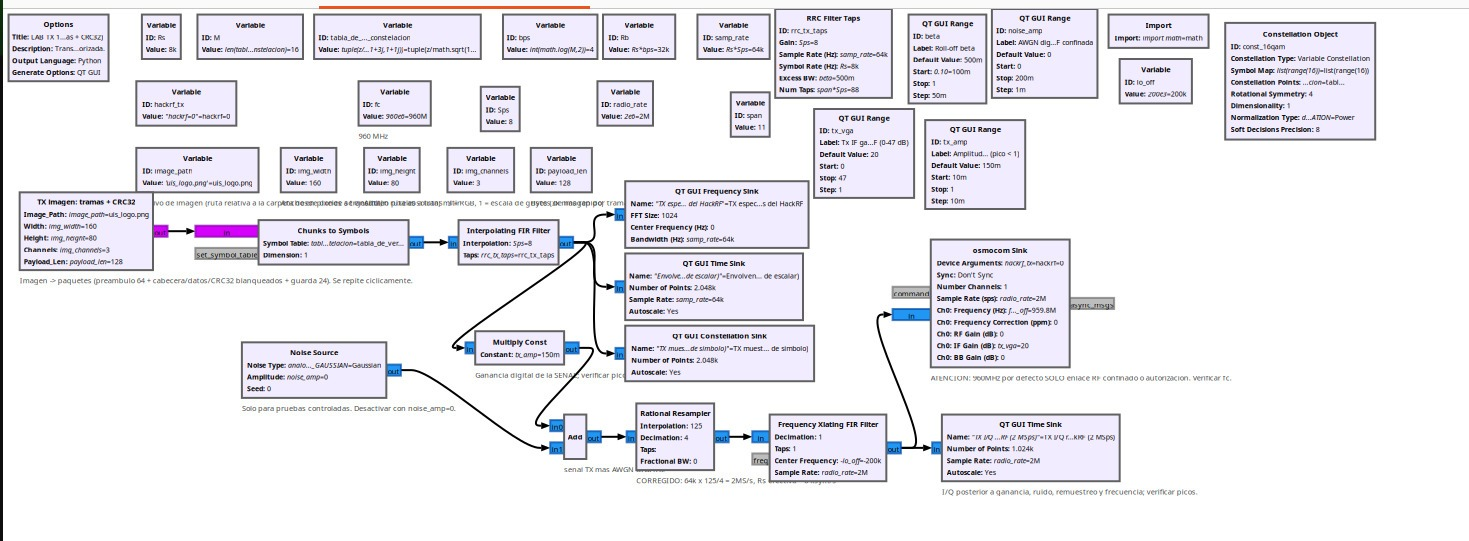
\includegraphics[width=0.95\textwidth]{figures/hardware_sdr/f4_tx_flujograma.jpg}
\caption{Flujograma del transmisor de imagen con HackRF One (\texttt{LAB\_TX\_16QAM\_HackRF\_IMAGEN.grc}).}
\label{fig:txflujo}
\end{figure*}

\begin{figure}[H]
\centering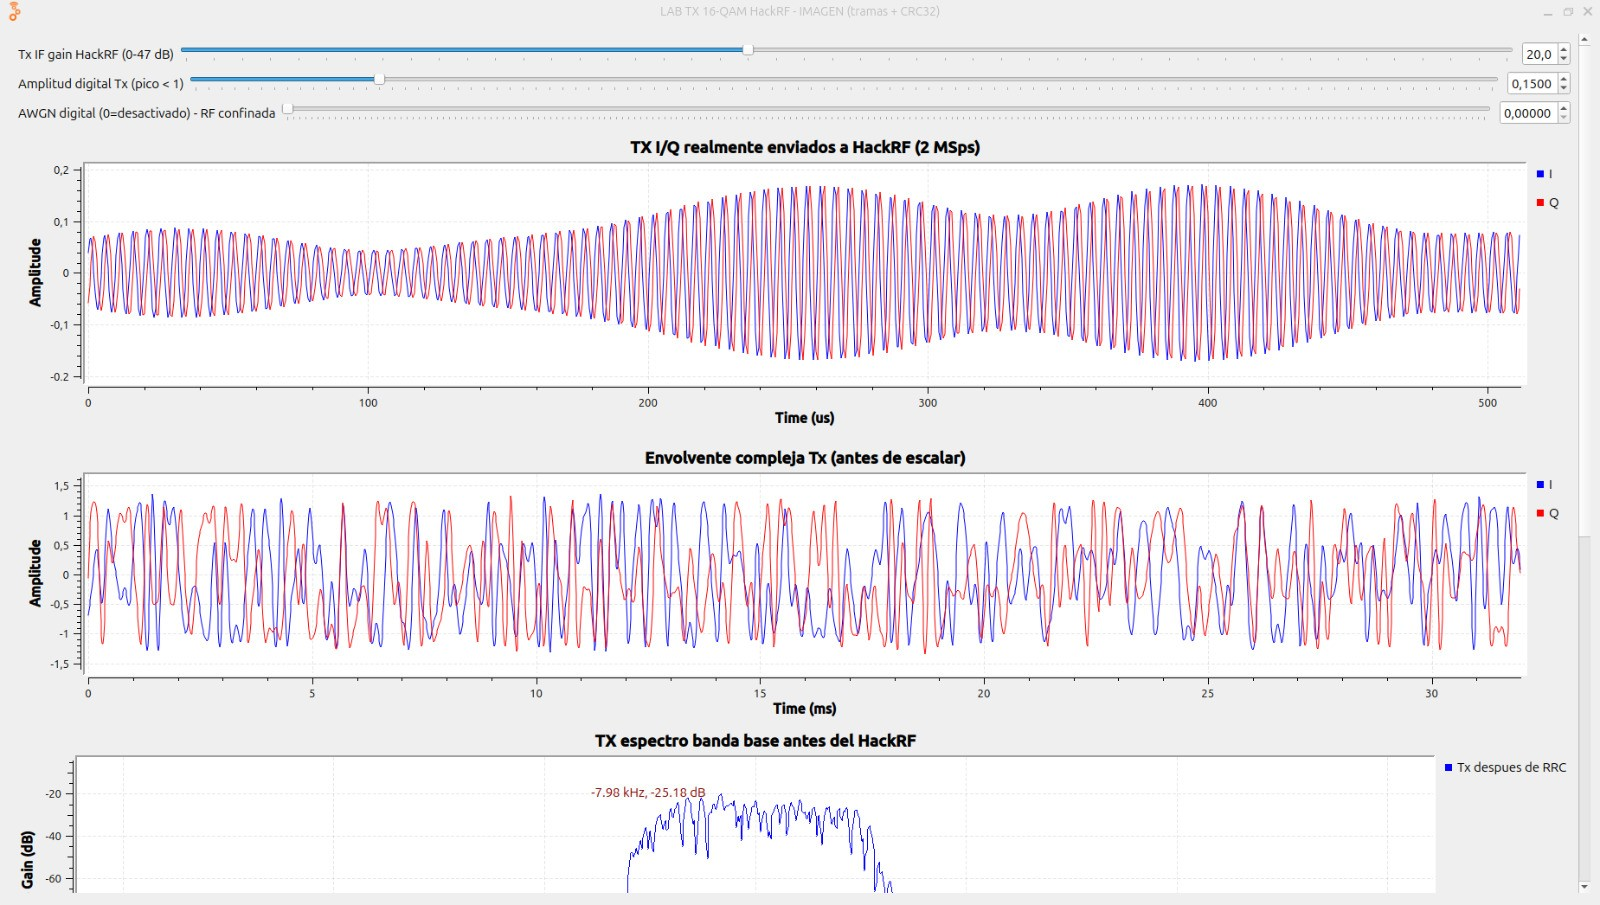
\includegraphics[width=\columnwidth]{figures/hardware_sdr/f4_tx_gui.jpg}
\caption{Interfaz del transmisor: I/Q enviada al HackRF (2~MS/s, desplazada 200~kHz), envolvente compleja antes de escalar y espectro tras el filtro RRC.}
\label{fig:txgui}
\end{figure}

\subsection{Prueba 1: mensaje ``El Pensador''}
El transmisor traía por defecto el texto ``LAB GNU RADIO 16QAM HACKRF 2026''; nuestro grupo lo cambió por ``El Pensador''. Con el texto la trama mide 192 símbolos (104 de datos).

Al iniciar, la constelación recuperada es una nube sin estructura (Fig.~\ref{fig:const}, izquierda): el FLL y el lazo de portadora aún no compensan el desfase entre los osciladores de los dos HackRF. A los pocos segundos aparecen los 16 grupos de la 16-QAM (Fig.~\ref{fig:const}, derecha). Los grupos están dispersos y algo deformados en las esquinas, lo que indica ruido y cierta compresión o ruido de fase.

\begin{figure*}[!t]
\centering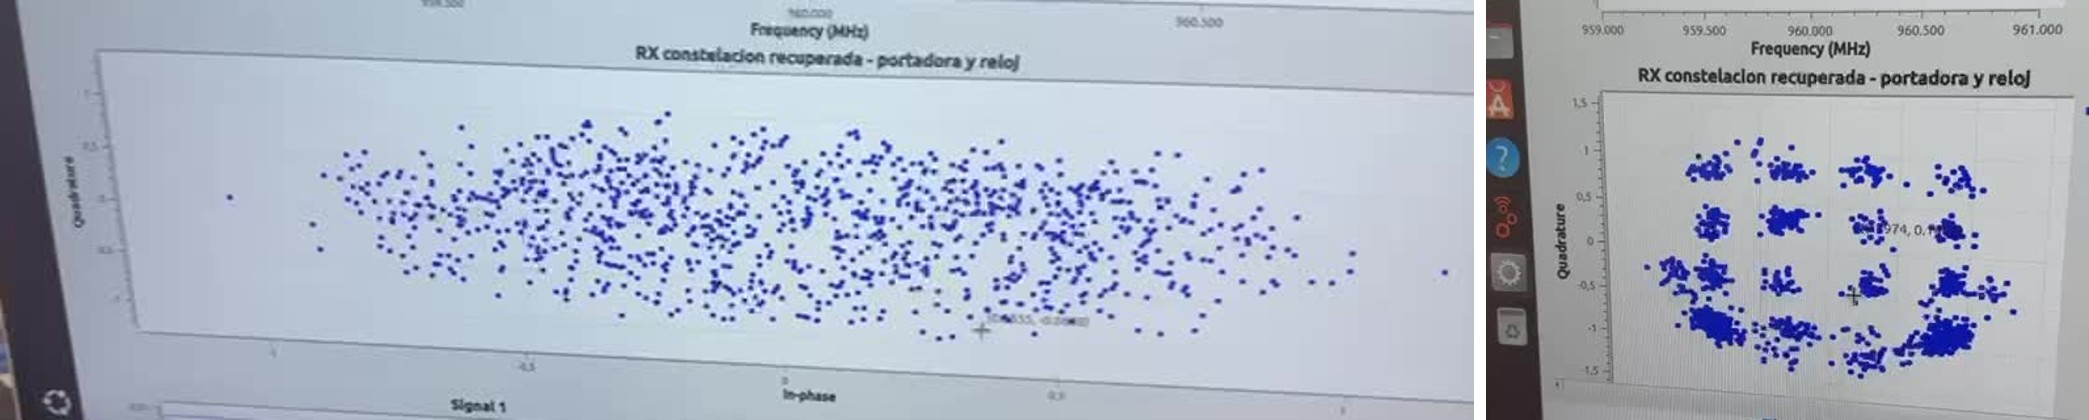
\includegraphics[width=0.92\textwidth]{figures/hardware_sdr/f4_constelacion.jpg}
\caption{Constelación recuperada con HackRF One. Izquierda: antes del enganche de portadora y reloj. Derecha: después, con los 16 puntos de la 16-QAM.}
\label{fig:const}
\end{figure*}

La consola (Fig.~\ref{fig:consola}) imprime cada 50 tramas la rotación detectada, el resultado del CRC y el texto. La mayoría de líneas muestran \texttt{CRC=OK, mensaje=El Pensador}: el mensaje llegó correcto. La rotación cambia entre 0, 90 y 180°, lo que confirma que el lazo de portadora se engancha en cualquiera de los cuatro giros de la 16-QAM y que el preámbulo resuelve esa ambigüedad. Algunas tramas dan \texttt{CRC=ERROR} con el texto alterado (``El Pefq!...''): el CRC detecta la trama corrupta y la descarta.

\begin{figure}[H]
\centering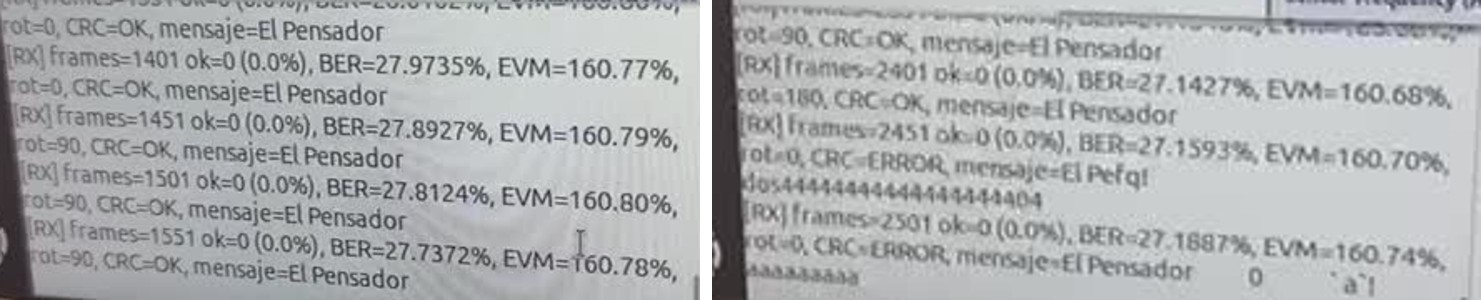
\includegraphics[width=\columnwidth]{figures/hardware_sdr/f4_consola_mensaje.jpg}
\caption{Consola del receptor en la prueba 1. Izquierda: tramas con CRC válido y el mensaje ``El Pensador''. Derecha: tramas con CRC=ERROR y texto alterado.}
\label{fig:consola}
\end{figure}

La consola también muestra $\texttt{ok}=0$, BER $\approx27.8$~\% y EVM $\approx160.8$~\%, casi constantes. Estos valores no describen el canal. El medidor calcula BER y EVM comparando contra la trama de referencia original, que conserva el texto ``LAB GNU RADIO 16QAM HACKRF 2026''. Al transmitir ``El Pensador'', lo que mide es la diferencia entre los dos textos. La calidad real del enlace la dan los CRC válidos, la constelación de 16 grupos y el EVM de la prueba 2.

\subsection{Prueba 2: imagen del logo UIS}
El transmisor cargó el logo de la UIS y lo redujo a 160$\times$80 píxeles RGB: 38\,400 bytes en 300 paquetes de 128 bytes. Cada paquete lleva una cabecera de 12 bytes con su número de secuencia, los datos y el CRC, blanqueados con una secuencia PRBS: $64+2(12+128+4)+24=376$ símbolos, es decir 47~ms. Los paquetes se repiten de forma cíclica, así que el receptor ubica cada paquete válido en su lugar aunque pierda otros.

La Fig.~\ref{fig:imagen} muestra el logo original y la imagen reconstruida. La imagen se forma por franjas horizontales verdes y blancas en la posición correcta: cada franja es un paquete con CRC válido (128 bytes $\approx$ 43 píxeles de una fila); lo negro son paquetes aún no recibidos. En el video se ve cómo aparecen franjas nuevas poco a poco.

\begin{figure}[H]
\centering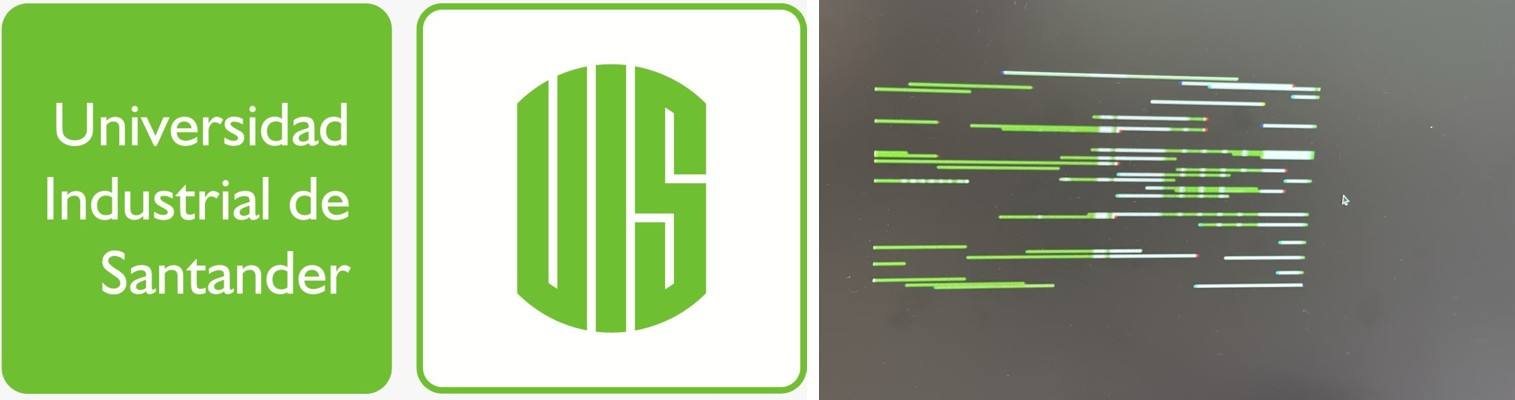
\includegraphics[width=\columnwidth]{figures/hardware_sdr/f4_imagen.jpg}
\caption{Izquierda: logo transmitido. Derecha: imagen reconstruida en el receptor, con los paquetes recibidos como franjas.}
\label{fig:imagen}
\end{figure}

La consola (Fig.~\ref{fig:consola2}) reporta, tras 19\,401 tramas, 52 con CRC válido (0.3~\%), el 15~\% de la imagen y un EVM de 16.7~\%. Aquí los datos de referencia coinciden con los transmitidos, así que el EVM sí describe la calidad de la señal.

\begin{figure}[H]
\centering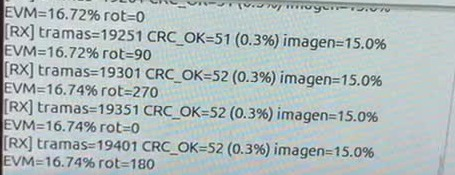
\includegraphics[width=0.85\columnwidth]{figures/hardware_sdr/f4_consola_imagen.jpg}
\caption{Consola del receptor en la prueba 2: tramas, CRC válidos, porcentaje de imagen y EVM.}
\label{fig:consola2}
\end{figure}

\subsection{Análisis de la prueba en hardware}
\textbf{Calidad de la señal.} Si el error fuera solo ruido gaussiano,
\begin{equation}
\mathrm{MER}\approx-20\log_{10}(\mathrm{EVM})=-20\log_{10}(0.167)\approx15.5~\mathrm{dB},
\end{equation}
y para 16-QAM con $E_s/N_0=15.5$~dB la probabilidad de error de símbolo es
\begin{equation}
P_s=1-\left[1-\tfrac{3}{2}Q\!\left(\sqrt{\tfrac{E_s}{5N_0}}\right)\right]^2\approx1.1\times10^{-2}.
\end{equation}

\textbf{Por qué el texto llegaba y la imagen no.} Una trama es válida solo si todos sus símbolos de datos son correctos: $P_{ok}=(1-P_s)^{n}$. Con el texto ($n=104$) resulta $P_{ok}\approx31$~\%; con la imagen ($n=288$), $P_{ok}\approx4$~\%. Por eso el mensaje corto aparecía con frecuencia y los paquetes de la imagen eran escasos.

\textbf{Pérdidas de sincronía.} Lo medido (0.27~\%) es unas 15 veces peor que esos 4~\%. El EVM solo se promedia sobre las tramas que el receptor detecta, así que no refleja los momentos de pérdida de enganche, los saltos de rotación ni los preámbulos no detectados. Atribuimos la diferencia a esas pérdidas de sincronía y al ruido de fase de los osciladores.

\textbf{Ritmo de reconstrucción.} Con 0.27~\% de tramas válidas y 47~ms por trama, llega un paquete bueno cada 17~s. Como los paquetes válidos caen al azar entre los 300, completar la imagen requeriría en promedio $300\,H_{300}\approx1885$ paquetes buenos, unas 9~h. El 15~\% observado en unos 15 minutos es coherente con ese ritmo.

\textbf{Relación con la simulación.} Como en el receptor BFSK simulado, la calidad de la detección depende de lo que ocurre antes del decisor: en la simulación, del ancho de banda de ruido que ve el discriminador; en hardware, de que FLL, reloj y portadora estén enganchados. Sin enganche no hay constelación útil, aunque la señal llegue con potencia suficiente.

\section{Conclusiones y trabajo futuro}
BFSK con $h=2$ satisface la telemetría de la planta con 10~kbit/s en unos 40~kHz y un receptor no coherente simple. El factor decisivo del receptor no es el decisor sino el ancho de banda que ve el discriminador: un filtro de selección de canal antes de la detección evita el efecto umbral y desplaza la curva de BER unos 13~dB. Con él, el enlace no presenta errores en las cuatro pruebas definidas.

La prueba con HackRF One llevó un enlace digital a un canal físico entre dos computadores. Tras el enganche de frecuencia, reloj y portadora, el receptor recuperó el mensaje ``El Pensador'' con CRC válido y resolvió la ambigüedad de fase de 90° mediante el preámbulo; el CRC-32 descartó las tramas corruptas. Con la imagen, un MER cercano a 15.5~dB hizo que pocos paquetes largos llegaran íntegros, y la reconstrucción avanzó por franjas hasta el 15~\%. El tamaño del paquete pesa tanto como la calidad de la señal, y las métricas de BER y EVM solo describen el canal cuando el receptor compara contra lo que realmente se transmitió.

Como trabajo futuro se propone: reemplazar Skip Head por Symbol Sync para tolerar errores de reloj; añadir corrección de desfase de frecuencia (AFC), que en Wireless M-Bus se exige por tolerancias de $\pm25$~ppm \cite{an0987}; evaluar GFSK para reducir lóbulos laterales; e incorporar ruido impulsivo de la maquinaria de bombeo.

\begin{thebibliography}{9}\footnotesize
\bibitem{proakis} J. G. Proakis y M. Salehi, \emph{Digital Communications}, 5.ª ed. New York, NY, USA: McGraw-Hill, 2008.
\bibitem{sklar} B. Sklar, \emph{Digital Communications: Fundamentals and Applications}, 2.ª ed. Upper Saddle River, NJ, USA: Prentice Hall, 2001.
\bibitem{an0987} A. Harney, ``Designing a wireless transceiver system to meet the Wireless M-Bus standard,'' Analog Devices, Norwood, MA, USA, Appl. Note AN-0987. [En línea]. Disponible: \url{https://www.analog.com/en/resources/app-notes/an-0987.html}
\bibitem{ahaneku} M. A. Ahaneku, ``FM threshold and methods of limiting its effect on performance,'' \emph{Nigerian J. Technol.}, vol. 26, no. 1, pp. 5--11, mar. 2007.
\bibitem{st_subghz} STMicroelectronics, ``Introduction to sub-1GHz,'' STM32 MCU Wiki. [En línea]. Disponible: \url{https://wiki.st.com/stm32mcu/wiki/Connectivity:Introduction_to_sub-1GHz}
\bibitem{hackrf} Great Scott Gadgets, ``HackRF One,'' documentación. [En línea]. Disponible: \url{https://hackrf.readthedocs.io}
\bibitem{gnuradio} GNU Radio Project, ``GNU Radio Manual and C++ API Reference / Block documentation.'' [En línea]. Disponible: \url{https://wiki.gnuradio.org}
\end{thebibliography}
\end{document}
